\section{One-dimensional grids}
\label{sec_one-dimensional}

One-dimensional grids ({\tt Grid1D}) are building blocks for three-dimensional 
computational domains ({\tt Domain}). A one-dimensional grid is a set of
points defined along a line segment, parallel to a particular coordinate 
direction. These points, usually referred to as {\em nodes}, divide the line 
segment in a number of smaller sub-segments, also called {\em cells}.
%
In the cell-centered finite volume method, used in {\psiboil} for 
discretization of governing equations, the unknowns are placed in centers
of the cells. 

\subsection{Uniform grid}
\label{sub_sec_uniform}

Imagine you want to create a one-dimensional grid, along the coordinate
axis~$\xi$, having length~$L=2.0$, starting at $\xi=-0.25 L$, ending 
at~$\xi=0.75 L$, divided in~16 cells. The cells have equal size, 
i.e.\ the grid is {\em uniform}. Such a grid can be created in {\psiboil}
with the following program ({\tt 05-01-main.cpp}):
%
{\small \begin{verbatim}
      1 #include "Include/psi-boil.h"
      2
      3 const real L = 2.0;
      4 const int  N = 16;
      5
      6 /****************************************************************************/
      7 main(int argc, char * argv[]) {
      8
      9   boil::timer.start();
     10
     11   /* non-periodic grid */
     12   Grid1D grid( Range<real>(-0.25*L, 0.75*L), N, Periodic::no());
     13
     14   // grid.print();
     15   // grid.plot("grid.eps");
     16
     17   boil::timer.stop();
     18   boil::timer.report();
     19 }
\end{verbatim}}
%
The grid is represented by the object {\tt grid}, and is defined in line~12. 
Program line~12 calls a constructor for grid, passing three parameters:
%
\begin{itemize}
  \item {\tt Range<real>(-0.25*L, 0.75*L)} - start and end $\xi$ coordinate of the grid,
  \item {\tt N}                            - number of grid cells ({\em not} nodes),
  \item {\tt Periodic::no()}               - indicator that the grid is non-periodic.
\end{itemize}
%
The first parameter sends the start and end $\xi$ coordinate, but they are
enclosed inside another object of type~{\tt Range}. As it's name implies,
{\tt Range} is a class which defines certain range, whether a range of
integer or real numbers\footnote{Actually it could be defined for any types
of objects which can be related with greater ({\tt >}), smaller ({\tt <})
or equal.}. Enclosing the starting and ending coordinate inside one object has
been done to group the similar items together (in one parameter) and, closely
connected with that, reduction of total number of parameters. 

Second parameter, {\tt N}, requires little explanation. It is an integer which
specifies number of cells in the grid.

Third parameter is a switch, telling {\tt Grid1D}'s constructor whether the grid
is periodic or not. It is passed with the special object of type {\tt Periodic},
which has only two member functions: {\tt yes()} and {\tt no()}. Their usage is
quite intuitive: If a grid is periodic, one would send {\tt Periodic::yes()} as
a parameter, and if it is not, one sends {\tt Periodic::no()}.

%----------------%
%                %
%  Uniform Grid  %
%                %
%----------------%
\begin{figure}[ht]
  \centering
  \setlength{\unitlength}{1mm}
  \begin{picture}(110,25)(0,0)
    \thickbox{110}{25}
    \put( 1,0){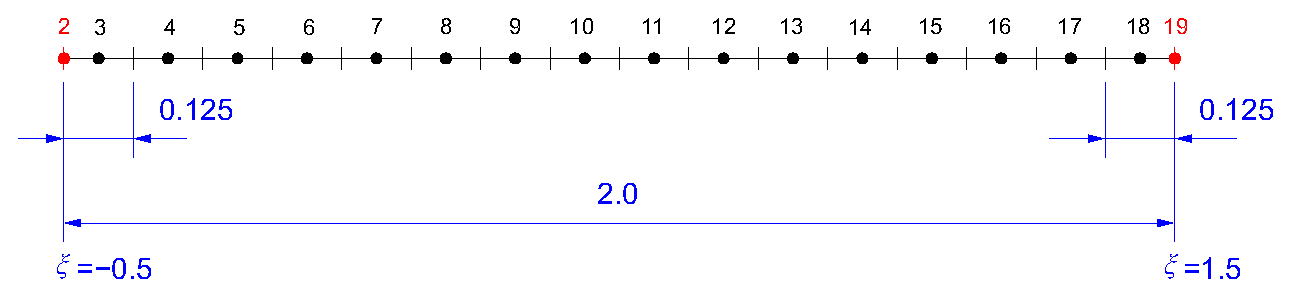
\includegraphics[scale=0.5]{Figures/05-01-grid.eps}}
  \end{picture}
  \caption{Uniform one-dimensional grid: 
                         $\bullet$ domain cells,
                         $+$       domain nodes,
                         \textcolor{red}{$\bullet$} boundary cells,
                         \textcolor{red}{$+$}       boundary nodes.
           Coordinates and dimensions are in blue.}
  \label{fig_uniform_grid}
\end{figure}

The grid created by this program is shown in Fig.~\ref{fig_uniform_grid}. 
First thing worth nothing is that there are~16 cells inside the domain (shown
by black dots and numbered from 1-16). But, in addition to cells in the
domain, {\psiboil} creates additional cells at the boundaries (red dots,
numbered 0 and 17). These {\em boundary} cells hold the values of boundary 
conditions or serve as {\em buffer} cells for parallel version. Note that,
for the case of non-periodic grid, boundary cells coincide with boundary
nodes.

If you would like to check all coordinates in the grid, un-comment line~14
and the program will write node, cell coordinates, as well as cell dimensions
on the terminal.
For a qualitative visual observation, un-comment line~15. The program will 
create an {\tt eps} figure in file {\tt grid.eps}. Both of these functions
({\tt print()} and {\tt plot(char * name)}) are used quite seldomly. Grid is
usually checked later in a post-processing package, after the {\tt Domain}
has been generated.

\subsection{Periodic grid}
\label{sub_sec_periodic}

If you want to create a periodic, line~12 from the above program should be 
changed to ({\tt 05-02-main.cpp}):
%
{\small \begin{verbatim}
     11   /* periodic grid */
     12   Grid1D grid( Range<real>(-0.25*L, 0.75*L), N, Periodic::yes());
\end{verbatim}}
%
This program, when compiled and ran, creates the grid shown in 
Fig.~\ref{fig_periodic_grid}. Dimensions of the domain cells are the same
as in previous example, but boundary cells do {\em not} coincide any
longer with boundary nodes. Boundary cell~0 is now a copy of domain
cell~16, shifted by $L$ in negative $\xi$ direction, while cell~17 is
a copy of cell~1, shifted by $L$ in positive $\xi$ direction. 

%-----------------%
%                 %
%  Periodic Grid  %
%                 %
%-----------------%
\begin{figure}[ht]
  \centering
  \setlength{\unitlength}{1mm}
  \begin{picture}(110,25)(0,0)
    \thickbox{110}{25}
    \put( 1,0){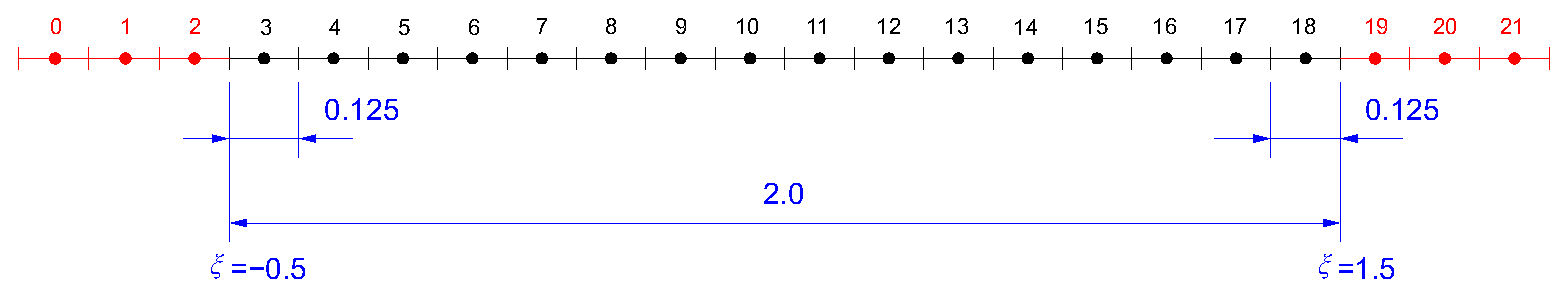
\includegraphics[scale=0.5]{Figures/05-02-grid.eps}}
  \end{picture}
  \caption{Periodic grid: $\bullet$ domain cells,
                          $+$       domain nodes,
                          \textcolor{red}{$\bullet$} boundary cells,
                          \textcolor{red}{$+$}       boundary nodes.
           Coordinates and dimensions are in blue.}
  \label{fig_periodic_grid}
\end{figure}

No matter if the grid is periodic or not, {\psiboil} adds additional cells
on the boundaries. The number of cells passed by the user, however, is 
equal to the number of {\em computational} cells. 

\subsection{Stretched grid}
\label{sub_sec_stretched}

The grids created in Sec\.~\ref{sub_sec_uniform} and~\ref{sub_sec_periodic}
were both uniform. Many problems require grid to be stretched towards
the regions where important phenomena is occurring at smaller scales to
resolve it more accurately. To create such {\em stretched} grids we need
to pass the desired cell dimension at the beginning and the end of the grid
to {\tt Grid1D}'s constructor. It is illustrated by the following program 
({\tt 05-03-main.cpp}):
%
{\small \begin{verbatim}
      1 #include "Include/psi-boil.h"
      2
      3 const real L  = 2.0;
      4 const real D1 = 0.002;
      5 const real D2 = 0.04;
      6 const int  N  = 32;
      7
      8 /****************************************************************************/
      9 main(int argc, char * argv[]) {
     10
     11   boil::timer.start();
     12
     13   /* stretched grid */
     14   Grid1D grid( Range<real>(-0.25*L, 0.75*L),
     15                Range<real>(D1, D2),
     16                N,
     17                Periodic::no());
     18
     19   grid.plot("grid.eps");
     20
     21   boil::timer.stop();
     22   boil::timer.report();
     23 }
\end{verbatim}}
%
Stretched grid is created by calling {\tt Grid1D} constructor in lines~14--17. 
Four parameters are passed to this constructor and they represent:
%
\begin{itemize}
  \item {\tt Range<real>(-0.25*L, 0.75*L)} - start and end $\xi$ coordinate of the grid,
  \item {\tt Range<real>(D1, D2)}          - start and end cell size of the grid,
  \item {\tt N}                            - number of grid cells ({\em not} nodes),
  \item {\tt Periodic::no()}               - indicator that the grid is non-periodic.
\end{itemize}
%
First, third and fourth parameter are the same as before, while second
parameter passes the desired start and end cell size. Grid created by
the program~({\tt 05-03-main.cpp}) is illustrated in Fig.~\ref{fig_stretched_grid}. 
As you can see, the grid is stretched towards both walls, with stretching
being stronger towards the beginning of the domain.

%------------------%
%                  %
%  Stretched Grid  %
%                  %
%------------------%
\begin{figure}[ht]
  \centering
  \setlength{\unitlength}{1mm}
  \begin{picture}(110,25)(0,0)
    \thickbox{110}{25}
    \put( 1,0){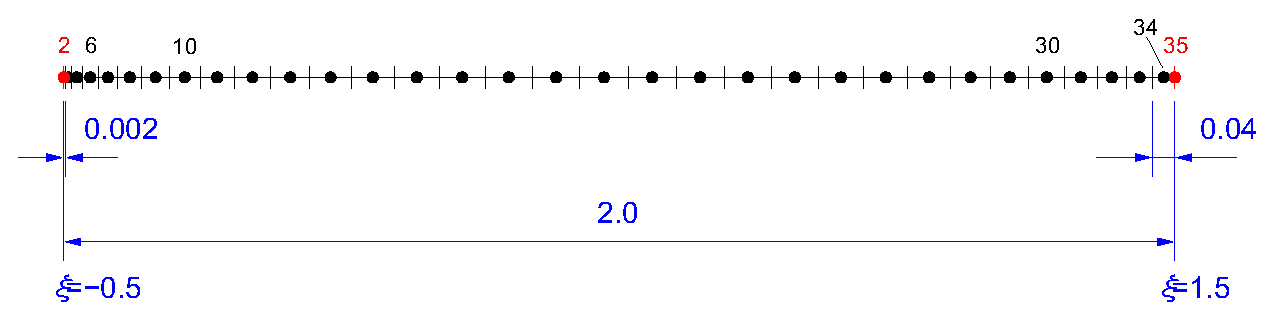
\includegraphics[scale=0.5]{Figures/05-03-grid.eps}}
  \end{picture}
  \caption{Stretched grid: $\bullet$ domain cells,
                           $+$       domain nodes,
                           \textcolor{red}{$\bullet$} boundary cells,
                           \textcolor{red}{$+$}       boundary nodes.
           Coordinates and dimensions are in blue.}
  \label{fig_stretched_grid}
\end{figure}

